\paragraph{QuizziPedia::Front-End::Directives::QuestionnaireResultsDirective}

\label{QuizziPedia::Front-End::Directives::QuestionnaireResultsDirective}

\begin{figure}[ht]
	\centering
	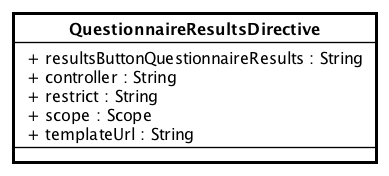
\includegraphics[scale=0.80,keepaspectratio]{UML/Classi/Front-End/QuizziPedia_Front-end_Directives_QuestionnaireResultsDirective.png}
	\caption{QuizziPedia::Front-End::Directives::QuestionnaireResultsDirective}
\end{figure} 
\FloatBarrier

\begin{itemize}
	\item \textbf{Descrizione}: rappresenta il componente grafico che permette all'utente autenticato pro di vedere i risultati di chi ha compilato il questionario. Tale componente è contenuto nella lista dei questionari abilitati alla compilazione. \'E possibile accedere alla lista dei risultati azionando l'evento ad esso collegato;
	\item \textbf{Utilizzo}: viene utilizzato per visualizzare i questionari abilitati alla compilazione e permettere all'utente di accedere alle statistiche ad essi associati;
	\item \textbf{Relazioni con altre classi}: 
	\begin{itemize} 
		\item \textbf{IN \texttt{QuizEventModelView}}: classe di tipo \textit{modelview\ped{G}} la cui istanziazione è contenuta all'interno della variabile di ambiente \$scope di \textit{Angular\ped{G}}. All'interno di essa sono presenti le variabili e i metodi necessari per il \textit{Two-Way Data-Binding\ped{G}} tra le \textit{directives\ped{G}} \texttt{EliminationAndModifyDirective}, \texttt{ExamModalityDirective} e \texttt{QuestionnaireResu-\\ltsDirective} e il \textit{controller\ped{G}} \texttt{QuizEventController};
		\item \textbf{IN \texttt{LangModel}}: rappresenta il modello delle informazioni per la giusta traduzione dell'applicazione;
		\item \textbf{OUT \texttt{QuestionnaireManagementView}}: \textit{view\ped{G}} principale per la gestione dei questionari.
	\end{itemize}
	\item \textbf{Attributi}: 
	\begin{itemize}
		\item \texttt{+ resultsButtonQuestionnaireResults: String} \\ Attributo che viene utilizzato per visualizzare la giusta traduzione della \textit{label\ped{G}} per il bottone di visualizzazione dei questionari, in italiano o in inglese;
		\item \texttt{+ controller: String} \\ Stringa contenente il nome del \textit{controller\ped{G}} della direttiva;
		\item \texttt{+ restrict: String} \\ Stringa che permette di definire le modalità di inserimento della direttiva all'interno della pagina;
		\item \texttt{+ scope: Scope} \\ Oggetto scope interno della direttiva, contiene le funzionalità per gestire i dati presenti all'interno;
		\item \texttt{+ templateUrl: String} \\ Stringa contenente il percorso del file \textit{HTML\ped{G}} che contiene la direttive.
	\end{itemize} 
\end{itemize}
